% LTeX: enabled=false
% Diapositivas de respaldo: solo se muestran si preguntan

% ===============================================================
% R1. Glosario
% ===============================================================
\begin{frame}{Respaldo: glosario}
    \begin{tabla}{colspec = {Q[l,m,4.4cm] X[l,m]}, rows = {font=\footnotesize}, rowsep = 1pt}
        Término & Qué significa \\
        Conjunto de datos (\textit{dataset}) & Estudios ya diagnosticados con los que aprende el modelo. \\
        Multimodal & Que combina distintos tipos de datos, en este caso imágenes y números. \\
        Red neuronal convolucional (CNN) & Tipo de modelo de IA que aprende a reconocer formas en imágenes. \\
        Grad-CAM & Marca qué zonas de la imagen pesaron más en el resultado. \\
        Falso negativo & Un ojo con queratocono que el modelo da como normal. Es el error a evitar. \\
        Sensibilidad & Porcentaje de ojos con queratocono que el modelo detecta. \\
        Validación & Probar el modelo con estudios que nunca vio. \\
    \end{tabla}
\end{frame}

% ===============================================================
% R2. Qué mide el equipo de la córnea
% ===============================================================
\begin{frame}{Respaldo: qué mide el equipo}
    \centering
    \resizebox{\linewidth}{!}{% Esquema de los parámetros corneales (Marco teórico)
% (a) corte de una córnea con queratocono sobre sus esferas de referencia
% (b) vista de frente: ubicación del punto más delgado y orientación en grados
\begin{tikzpicture}[
    font=\small,
    >={Stealth[length=1.8mm]},
    referencia/.style = {dashed, gray!70, thick},
    superficie/.style = {very thick, black!80},
    cota/.style = {<->, thick},
    nota/.style = {font=\footnotesize, align=left, inner sep=1pt,
                   execute at begin node={\setstretch{1}}},
    guia/.style = {thin},
    declare function={
        esfAnt(\x) = sqrt(36 - \x*\x) - 3;          % esfera de referencia anterior
        esfPos(\x) = sqrt(27.04 - \x*\x) - 2.8;     % esfera de referencia posterior
        cono(\x)   = exp(-((\x - 0.8)^2) / 1.6);    % protrusión del cono
        ant(\x)    = esfAnt(\x) + 0.6*cono(\x) - 0.1;
        pos(\x)    = esfPos(\x) + 0.9*cono(\x) - 0.1;
    }
  ]

  % ---------------- (a) Corte de la córnea ----------------
  % Tejido corneal entre ambas superficies
  \fill[blue!10]
    plot[domain=-4:4, samples=120] (\x, {ant(\x)})
    -- plot[domain=4:-4, samples=120] (\x, {pos(\x)}) -- cycle;
  % Esferas de referencia (forma ideal)
  \draw[referencia] plot[domain=-4.2:4.2, samples=80] (\x, {esfAnt(\x)});
  \draw[referencia] plot[domain=-4.2:4.2, samples=80] (\x, {esfPos(\x)});
  % Superficies reales
  \draw[superficie] plot[domain=-4:4, samples=120] (\x, {ant(\x)});
  \draw[superficie] plot[domain=-4:4, samples=120] (\x, {pos(\x)});
  \node[nota] at (-3.2, 2.75) {cara anterior};
  \node[nota] at (-2.0, 1.2) {cara posterior};

  % Zona de 3 mm centrada en el punto más delgado (A y B)
  \draw[orange!80!black, thick, |-|] (-0.15, 4.15) -- (1.75, 4.15)
    node[midway, above=2pt, nota, text=orange!80!black] {zona de 3 mm (A y B)};
  \draw[orange!80!black, densely dotted] (-0.15, 4.15) -- (-0.15, {ant(-0.15)});
  \draw[orange!80!black, densely dotted] (1.75, 4.15) -- (1.75, {ant(1.75)});

  % K max: punto de mayor curvatura de la cara anterior
  \fill[violet] (0.8, {ant(0.8)}) circle (2.2pt);
  \node[nota, text=violet] (lkmax) at (-3.1, 4.3) {\textbf{K max}: punto de mayor\\curvatura de la cara anterior};
  \draw[guia, violet] (lkmax.east) -- (0.75, {ant(0.8)+0.05});

  % Espesor mínimo (C)
  \draw[cota, teal!70!black] (0.8, {pos(0.8)}) -- (0.8, {ant(0.8)});
  \node[nota, text=teal!70!black] (lesp) at (5.6, 3.7) {\textbf{Espesor mínimo (C)}:\\espesor en el punto\\más delgado};
  \draw[guia, teal!70!black] (lesp.west) -- (0.85, {(ant(0.8)+pos(0.8))/2});

  % Elevaciones respecto de las esferas de referencia
  \draw[cota, red!70!black] (1.75, {esfAnt(1.75)}) -- (1.75, {ant(1.75)});
  \draw[cota, red!70!black] (1.75, {esfPos(1.75)}) -- (1.75, {pos(1.75)});
  \node[nota, text=red!70!black] (lelev) at (5.6, 2.1) {\textbf{Elevación} anterior\\y posterior: cuánto\\sobresale cada cara\\de su esfera};
  \draw[guia, red!70!black] (lelev.west) -- (1.8, {(esfAnt(1.75)+ant(1.75))/2});
  \draw[guia, red!70!black] (lelev.west) -- (1.8, {(esfPos(1.75)+pos(1.75))/2});

  % Leyenda
  \draw[referencia] (-4, 0.15) -- ++(0.6, 0) node[right, nota, text=black] {esfera de referencia (forma ideal)};
  \fill[blue!10] (-4, -0.45) rectangle ++(0.6, 0.3);
  \node[nota, right] at (-3.3, -0.3) {tejido corneal};
  \node[font=\small\bfseries] at (0.6, -1.05) {(a) Corte de una córnea con queratocono};
  \node[nota, text=gray] at (0.6, -1.5) {Esquema sin escala: las deformaciones están exageradas.};

  % ---------------- (b) Vista de frente ----------------
  \begin{scope}[shift={(10.6, 2.0)}]
    \fill[blue!6] (0,0) circle (2.1);
    \draw[thick] (0,0) circle (2.1);
    \draw[gray!60] (-2.35,0) -- (2.35,0);
    \draw[gray!60] (0,-2.35) -- (0,2.35);
    \node[nota] at (2.65, 0) {0°};
    \node[nota] at (-2.8, 0) {180°};
    \node[nota] at (0, 2.6) {90°};
    % Dos orientaciones casi iguales: 1° y 179°
    \draw[red!70!black, thick] (0,0) -- (1:2.1) node[pos=0.72, above=1pt, nota, text=red!70!black] {1°};
    \draw[red!70!black, thick, dashed] (0,0) -- (179:2.1) node[pos=0.72, above=1pt, nota, text=red!70!black] {179°};
    % Punto más delgado, su ubicación (x, y) y la zona de 3 mm
    \coordinate (pmd) at (0.55, -0.85);
    \draw[orange!80!black, thick] (pmd) circle (0.7);
    \draw[teal!70!black, densely dotted] (pmd) -- (0.55, 0) node[above, nota, text=teal!70!black] {$x$};
    \draw[teal!70!black, densely dotted] (pmd) -- (0, -0.85) node[left, nota, text=teal!70!black] {$y$};
    \fill[teal!70!black] (pmd) circle (2.2pt);
    \node[nota, align=center] at (0, -2.85) {\textcolor{teal!70!black}{punto más delgado en $(x, y)$}\\\textcolor{orange!80!black}{y zona de 3 mm a su alrededor}};
    \node[nota, align=center, text=red!70!black] at (0, 3.15) {1° y 179° marcan casi\\la misma dirección};
    \node[font=\small\bfseries] at (0, -3.05) [below=8pt] {(b) Vista de frente};
  \end{scope}
\end{tikzpicture}
}
\end{frame}

% ===============================================================
% R3. Detalle del análisis exploratorio
% ===============================================================
\begin{frame}{Respaldo: datos clínicos por grupo}
    \centering
    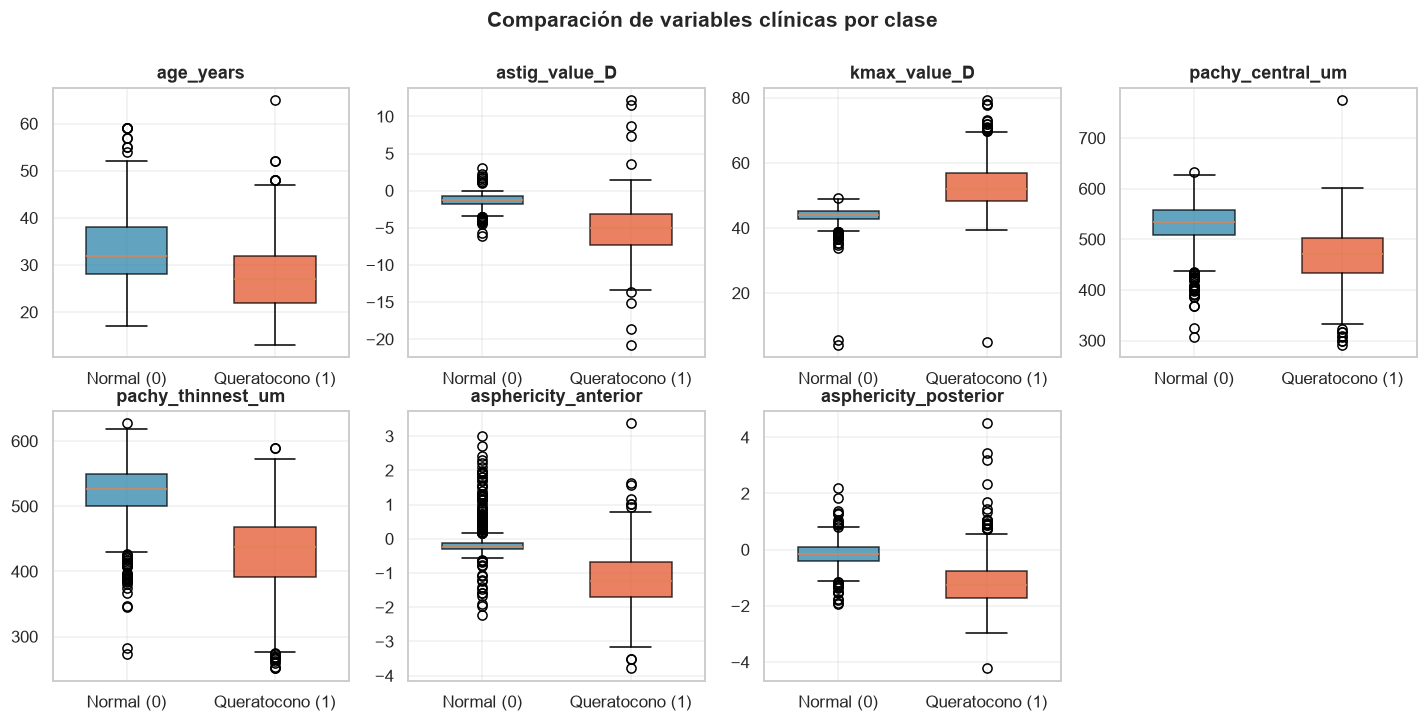
\includegraphics[width=0.82\linewidth]{eda/eda_variables_clinicas.png}\par
    {\small Cada caja muestra la mitad central de los valores de cada grupo, normal y con queratocono.}
\end{frame}
